\documentclass[12pt]{article}
\usepackage{graphicx}
\usepackage[margin=1in]{geometry}
\usepackage{caption}
\usepackage{xcolor}
\usepackage{float}
\usepackage{amsmath}
\usepackage{array}
\usepackage{multicol}
\usepackage{hyperref}
\usepackage{url}
\usepackage{listings}
\usepackage{courier}

\lstset{
  basicstyle=\ttfamily\footnotesize,
  backgroundcolor=\color{gray!10},
  frame=single,
  breaklines=true,
  captionpos=b
}

\setlength{\columnsep}{1cm}

\begin{document}

% Title Block
\begin{figure}[H]
    \begin{minipage}{0.45\textwidth}
        \includegraphics[width=\textwidth]{iiitb_comet.jpeg} % Replace with your logo
    \end{minipage} \hfill
    \begin{minipage}{0.45\textwidth}
        \textbf{Name: S.Rithrishareddy} \\
        \textbf{Batch: COMETFWC028} \\
        \textbf{Date: 03 June 2025}
    \end{minipage}
\end{figure}

\begin{center}
    {\LARGE \textbf{\textcolor{cyan}{GATE 2009, ECE Question Number 39}}}
\end{center}
\vspace{1em}

\begin{multicols}{2}

\noindent\textbf{Abstract} \\[0.5em]
This project implements the JK Flip-Flop-based 3-state counter problem from GATE 2009 Q39 using Raspberry Pi Pico W. Through simulation of JK flip-flop behavior, button-triggered clock inputs change the output state, which is observed on two LEDs representing Q1 and Q2. This project demonstrates how sequential logic circuits can be modeled using embedded hardware and MicroPython programming.

\begin{figure}[H]
    \centering
    \includegraphics[width=0.6\linewidth]{jk_flipflop.png} % Replace with JK FF logic diagram
    \caption*{Figure: JK Flip-Flop logic diagram used in simulation}
\end{figure}

\vspace{1em}
\noindent\textbf{1. Components}
\begin{table}[H]
\small
\centering
\begin{tabular}{|p{4.2cm}|c|}
\hline
\textbf{Component} & \textbf{Qty} \\
\hline
Raspberry Pi Pico W & 1 \\
Push Button (clock input) & 1 \\
LEDs (Q1, Q2) & 2 \\
220$\Omega$ Resistors & 2 \\
Breadboard & 1 \\
Jumper Wires & 8 \\
Micro-USB Cable & 1 \\
\hline
\end{tabular}
\caption*{Table 1: List of components used}
\end{table}

\vspace{1em}
\noindent\textbf{2. Setup and Connections}
\begin{itemize}
    \item \textbf{Button (Clock)} → GPIO 15 with a pull-down resistor.
    \item \textbf{LED Q1} → GPIO 16 via 220$\Omega$ resistor.
    \item \textbf{LED Q2} → GPIO 17 via 220$\Omega$ resistor.
    \item GND connections from Pico to breadboard.
    \item Button press triggers state change.
\end{itemize}

\vspace{1em}
\noindent\textbf{3. State Table for Q39}
\begin{table}[H]
\centering
\begin{tabular}{|c|c|c|}
\hline
\textbf{Press} & \textbf{Q2} & \textbf{Q1} \\
\hline
Initial & 0 & 0 \\
1st     & 0 & 1 \\
2nd     & 1 & 0 \\
3rd     & 0 & 0 \\
4th     & 0 & 1 \\
\hline
\end{tabular}
\caption*{Table 2: State transition sequence for 3-state counter}
\end{table}

\end{multicols}

\newpage

\section*{4. Analysis}
\begin{itemize}
    \item Flip-Flop 1 toggles on every clock (J=Q2, K=1)
    \item Flip-Flop 2 toggles based on Q1 (J=Q1, K=1)
    \item Implemented logic replicates JK Flip-Flop transitions
    \item LED outputs match the cyclic state sequence: 01 → 10 → 00 → ...
\end{itemize}

\section*{5. Circuit Image}
\begin{figure}[H]
    \centering
    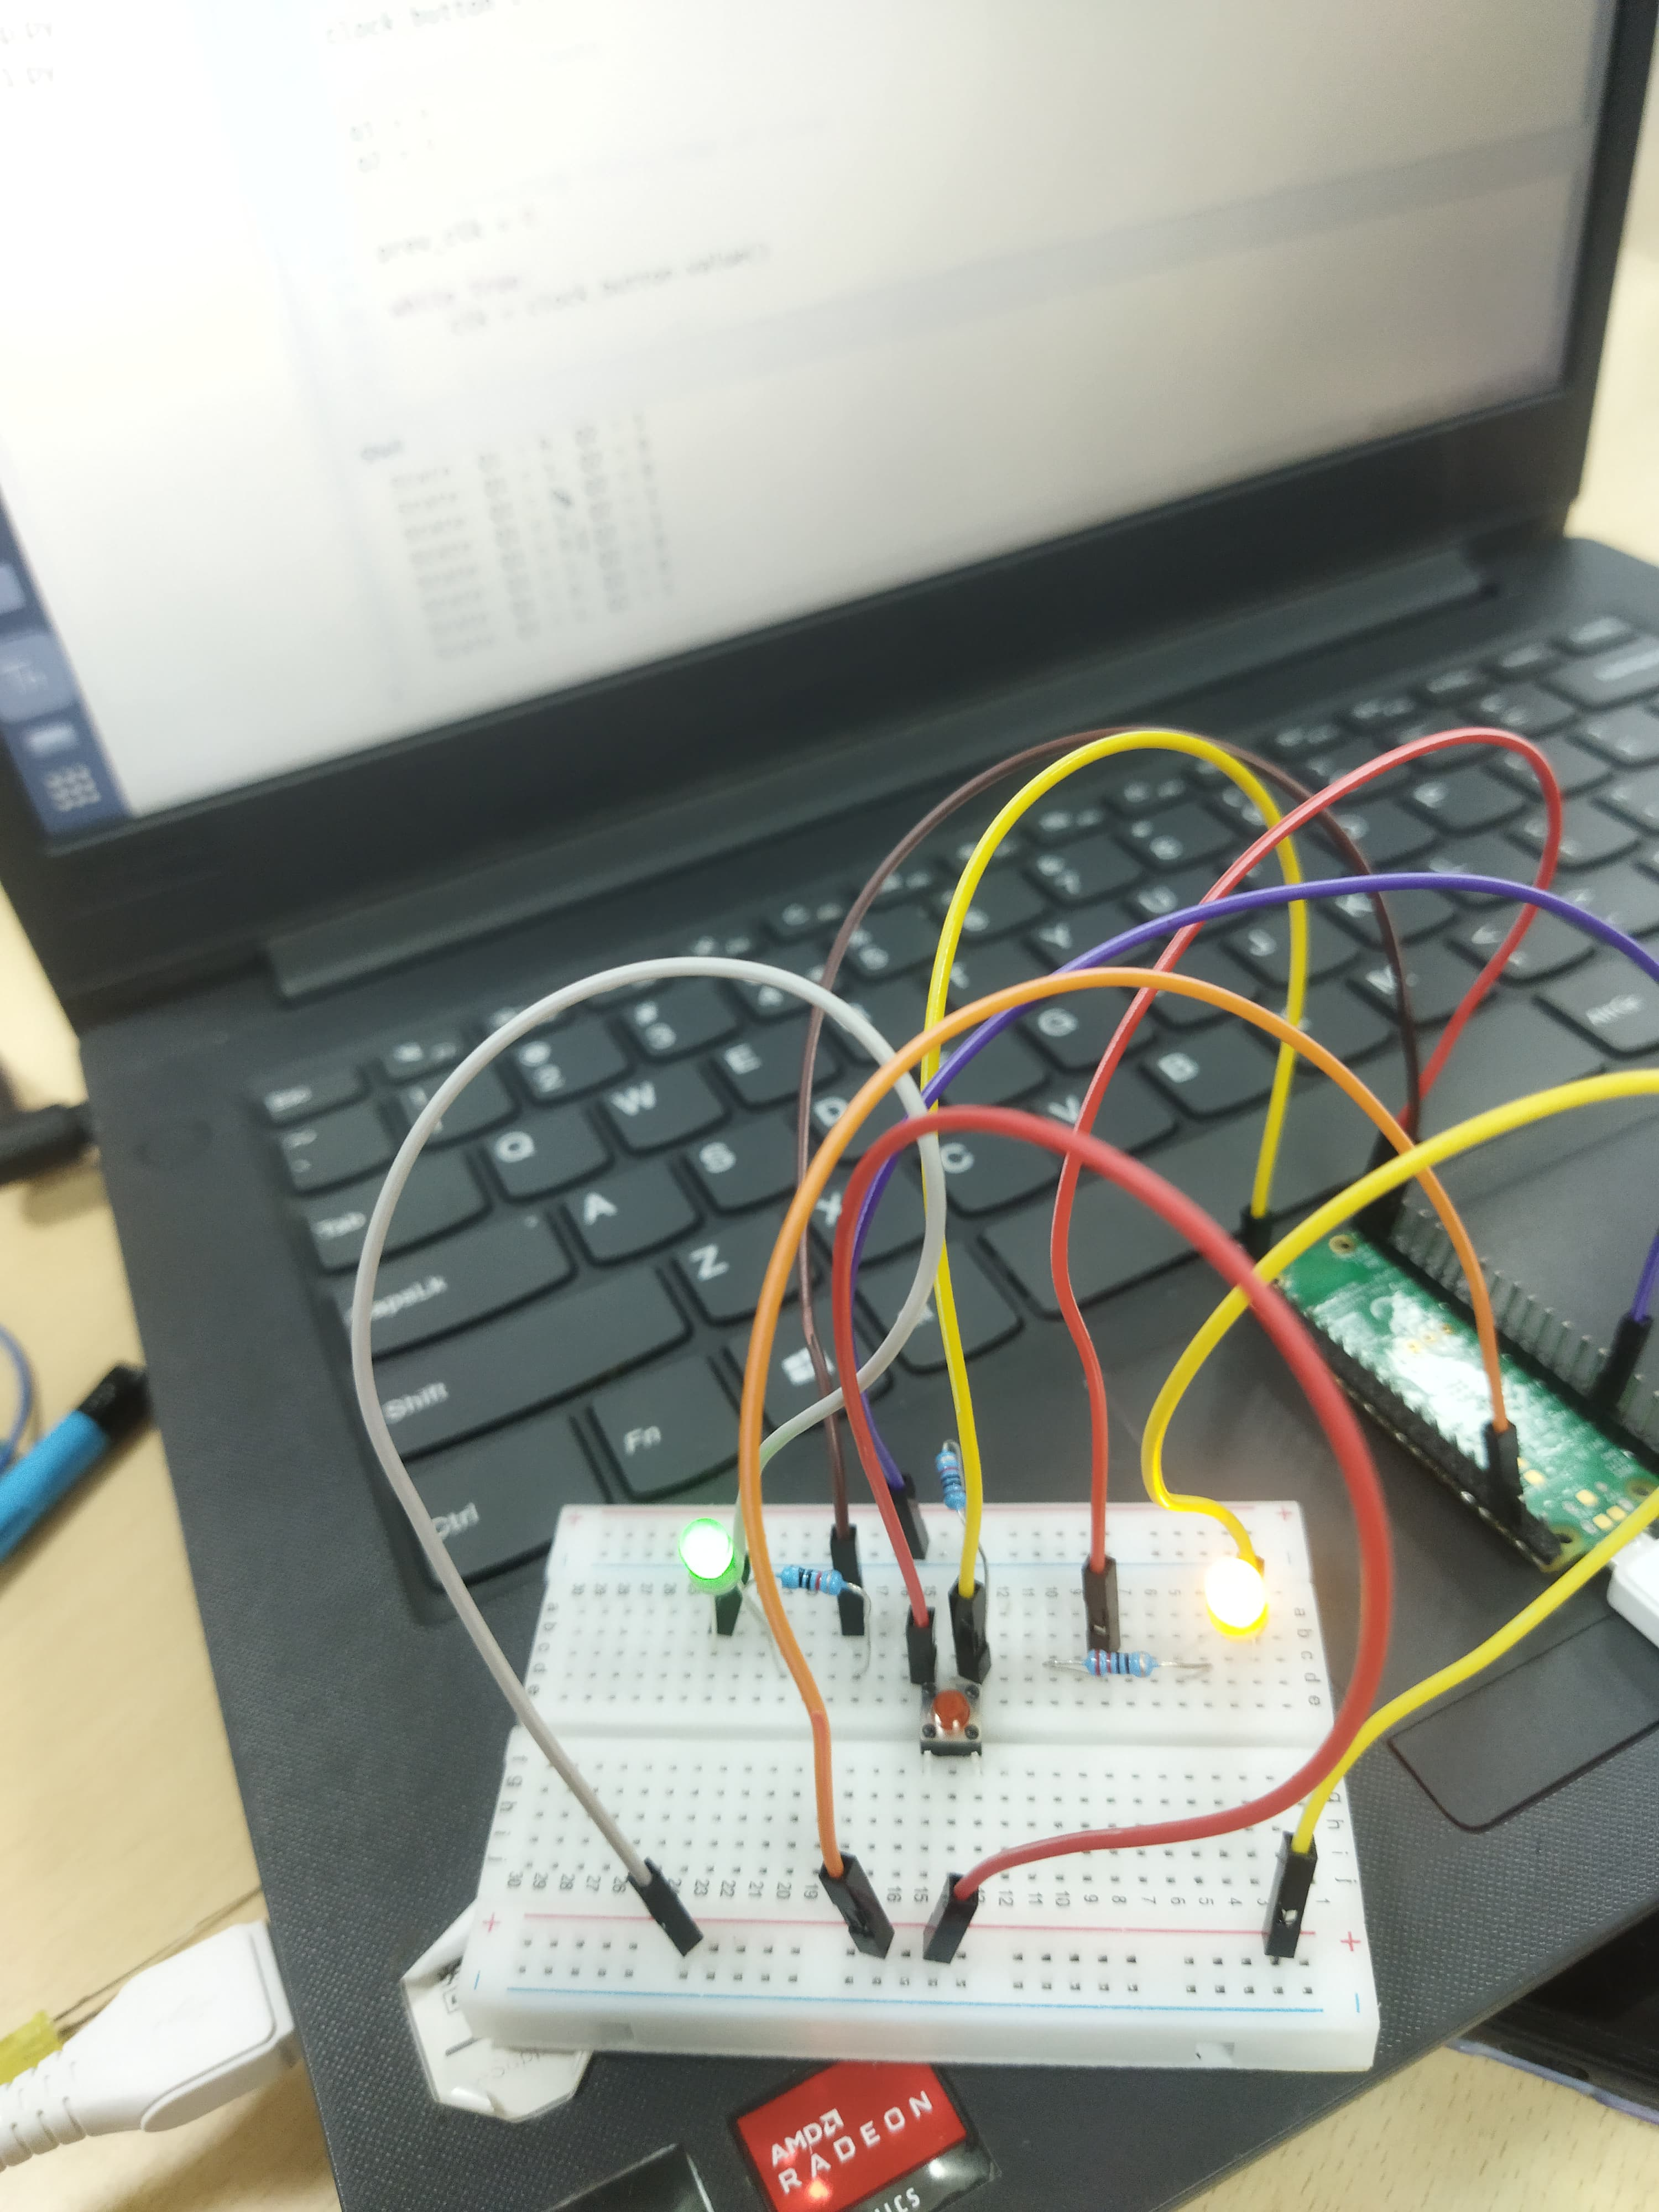
\includegraphics[width=0.7\linewidth]{esp32.jpeg} % Replace with actual hardware image
    \caption*{Figure: Real hardware setup using Raspberry Pi Pico W}
\end{figure}

\section*{6. Conclusion}
This hardware implementation using Raspberry Pi Pico W accurately simulates the JK flip-flop logic as described in GATE ECE 2009 Q39. It clearly demonstrates the principles of sequential logic and state transitions through LED outputs. This experiment helps bridge theoretical flip-flop concepts with practical embedded systems. The modularity of Pico W also makes the solution scalable for more complex digital systems.

\section*{7. GitHub Repository}
\begin{itemize}
    \item Project code and documentation: \\
    \url{https://github.com/Rithrishareddy/RITHRISHA_FWC/tree/main/Hardware}
\end{itemize}

\section*{8. Learning Outcomes}
\begin{itemize}
    \item Gained hands-on experience with JK flip-flop implementation on real hardware.
    \item Understood sequential circuit behavior through state transitions.
    \item Practiced GPIO pin configuration, debouncing techniques, and LED state control.
    \item Learned to simulate theoretical counters in a hardware-based environment.
    \item Improved MicroPython programming and debugging skills on embedded platforms.
\end{itemize}

\end{document}
